\chapter{PLANOS Y LAMINAS DE DETALLE}

Los planos deben colocarse en la carpeta:

\begin{center}
\texttt{latex/planos/}
\end{center}

Cuando cada plano exista en PDF o imagen, debe guardarse con el nombre indicado y actualizarse el estado de la tabla.

\begin{landscape}
\begin{longtable}{L{1.6cm}L{3.3cm}L{4.3cm}L{1.8cm}}
\caption{Relacion de planos requeridos}\label{tab:planos}\\
\toprule
\textbf{Codigo} & \textbf{Plano} & \textbf{Archivo esperado} & \textbf{Estado} \\
\midrule
\endfirsthead
\toprule
\textbf{Codigo} & \textbf{Plano} & \textbf{Archivo esperado} & \textbf{Estado} \\
\midrule
\endhead
IE-01 & Ubicación y arquitectura/croquis & \shortstack[l]{primer-piso.pdf\\segundo-piso.pdf\\tercer-piso.pdf} & Entregado \\
IE-02 & Instalaciones Eléctricas - Alumbrado & \shortstack[l]{IE-02-\\alumbrado.pdf} & Entregado \\
IE-03 & Instalaciones Eléctricas - Tomacorrientes & \shortstack[l]{IE-03-\\tomacorrientes.pdf} & Entregado \\
IE-04 & Instalaciones Eléctricas - Canalizaciones & \shortstack[l]{IE-04-circuitos-\\canalizaciones.pdf} & Entregado \\
IE-05 & Diagrama unifilar y cuadro de cargas & \shortstack[l]{IE-05-unifilar-\\cuadro-cargas.pdf} & Entregado \\
IE-06 & Puesta a tierra & \shortstack[l]{IE-06-\\puesta-tierra.pdf} & Entregado \\
IE-07 & Simbología y detalles eléctricos & \shortstack[l]{IE-07-simbologia-\\detalles.pdf} & Entregado \\
\bottomrule
\end{longtable}
\end{landscape}

\section{Planos a insertar}

\subsection{IE-01: Ubicación y arquitectura}

A continuación, se presentan los planos de distribución arquitectónica de la vivienda para cada uno de los tres pisos, generados mediante la herramienta local.

\begin{landscape}
\begin{figure}[H]
  \centering
  
\includegraphics[height=0.82\textheight,keepaspectratio]{planos/primer-piso.pdf}
  \caption{Plano de Distribución Arquitectónica - Primer Piso}
  \label{fig:arq-primer-piso}
\end{figure}
\end{landscape}

\begin{landscape}
\begin{figure}[H]
  \centering
  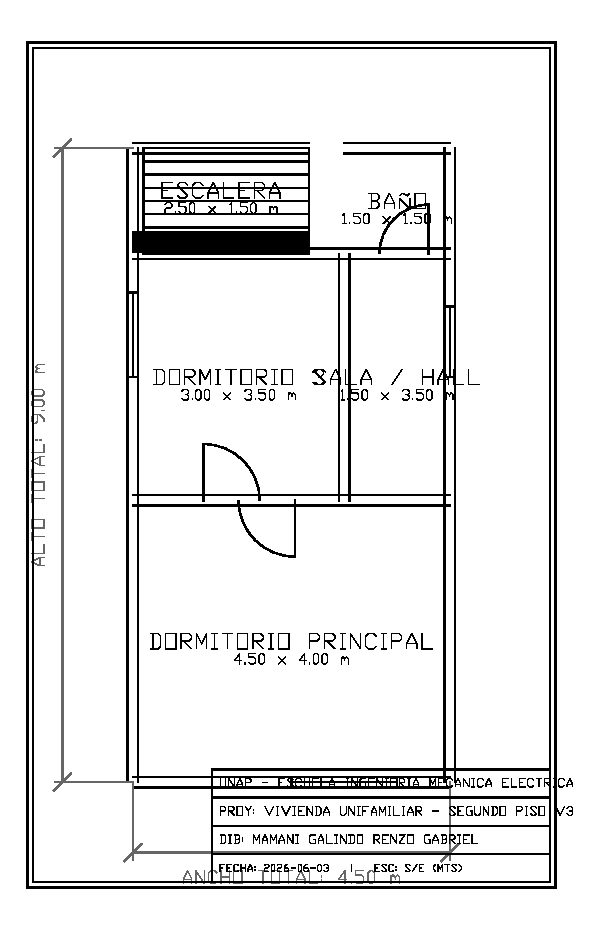
\includegraphics[height=0.82\textheight,keepaspectratio]{planos/segundo-piso.pdf}
  \caption{Plano de Distribución Arquitectónica - Segundo Piso}
  \label{fig:arq-segundo-piso}
\end{figure}
\end{landscape}

\begin{landscape}
\begin{figure}[H]
  \centering
  
\includegraphics[height=0.82\textheight,keepaspectratio]{planos/tercer-piso.pdf}
  \caption{Plano de Distribución Arquitectónica - Tercer Piso}
  \label{fig:arq-tercer-piso}
\end{figure}
\end{landscape}


\subsection{IE-02: Instalaciones Eléctricas - Alumbrado (3 Pisos)}

A continuación se presenta el diseño de alumbrado para los tres niveles de la vivienda unifamiliar, conteniendo la distribución de luminarias LED, interruptores simples y de conmutación (tres vías) y las canalizaciones de alumbrado correspondientes.

\begin{landscape}
\begin{figure}[H]
  \centering
  
\includegraphics[height=0.82\textheight,keepaspectratio]{planos/IE-02-alumbrado.pdf}
  \caption{Plano de Instalaciones Eléctricas - Alumbrado (Consolidado)}
  \label{fig:instalaciones-alumbrado}
\end{figure}
\end{landscape}

\subsection{IE-03: Instalaciones Eléctricas - Tomacorrientes (3 Pisos)}

A continuación se presenta el diseño de tomacorrientes para los tres niveles de la vivienda unifamiliar, conteniendo los tomacorrientes generales y especiales (para cocina, lavandería y bomba de agua) y las respectivas canalizaciones.

\begin{landscape}
\begin{figure}[H]
  \centering
  
\includegraphics[height=0.82\textheight,keepaspectratio]{planos/IE-03-tomacorrientes.pdf}
  \caption{Plano de Instalaciones Eléctricas - Tomacorrientes (Consolidado)}
  \label{fig:instalaciones-tomacorrientes}
\end{figure}
\end{landscape}

\subsection{IE-04: Instalaciones Eléctricas - Circuitos y Canalizaciones (3 Pisos)}

A continuación se presenta el diseño integral de circuitos y canalizaciones para los tres niveles de la vivienda unifamiliar, conteniendo la distribución de tableros, medidores, pozo a tierra y las rutas eléctricas generales.

\begin{landscape}
\begin{figure}[H]
  \centering
  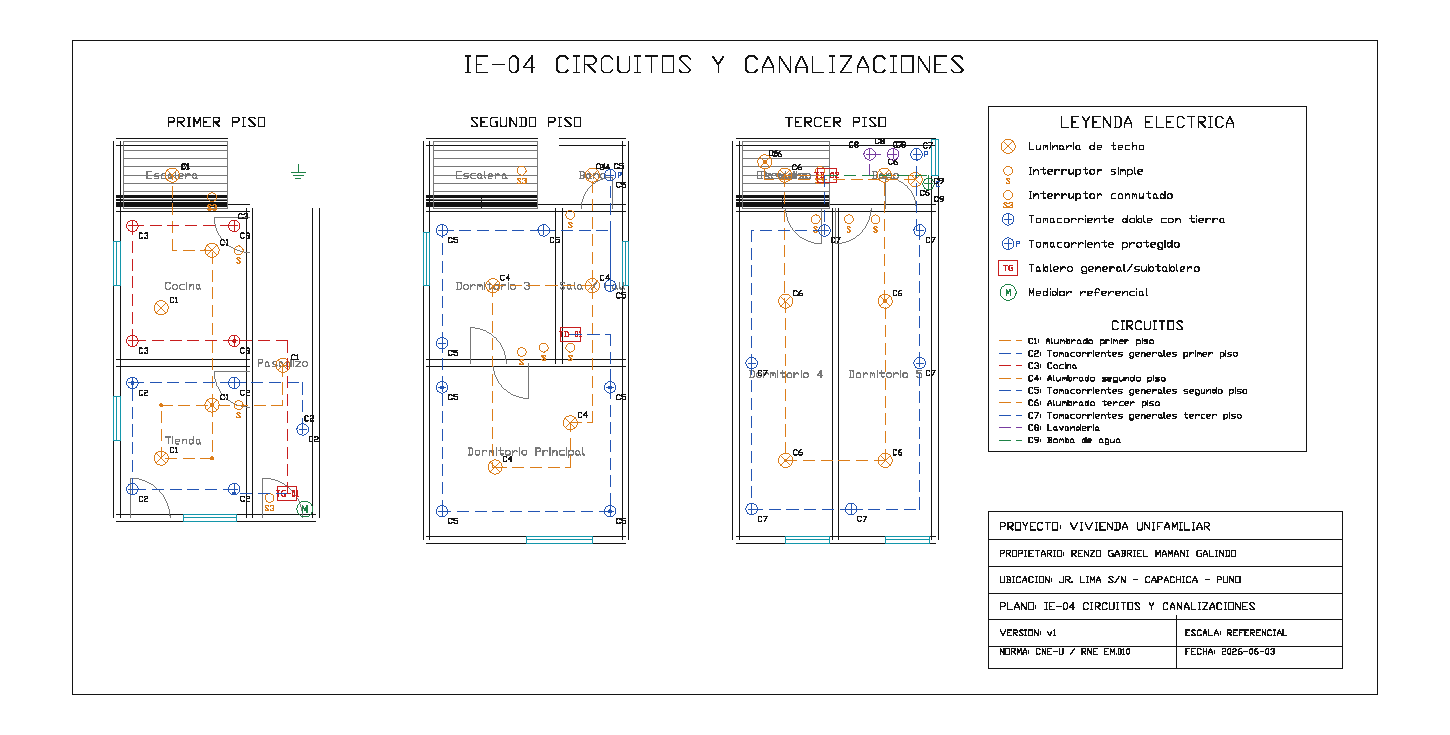
\includegraphics[height=0.82\textheight,keepaspectratio]{planos/IE-04-circuitos-canalizaciones.pdf}
  \caption{Plano de Instalaciones Eléctricas - Circuitos y Canalizaciones (Consolidado)}
  \label{fig:instalaciones-canalizaciones}
\end{figure}
\end{landscape}

\subsection{IE-05: Diagrama Unifilar y Cuadro de Cargas}

A continuación se presenta el diagrama unifilar general de la vivienda unifamiliar, detallando las capacidades de interrupción de los termomagnéticos y diferenciales para el tablero general TG-01, los tableros secundarios de distribución TD-01 y TD-02, y el cuadro general de cargas actualizado con 6 circuitos.

\begin{landscape}
\begin{figure}[H]
  \centering
  
\includegraphics[height=0.82\textheight,keepaspectratio]{planos/IE-05-unifilar-cuadro-cargas.pdf}
  \caption{Diagrama Unifilar General de la Vivienda y Subtableros}
  \label{fig:diagrama-unifilar-gral}
\end{figure}
\end{landscape}

\subsection{IE-06: Puesta a Tierra y Detalles de Conexión}

Se detalla la conexión de puesta a tierra desde la barra del tablero general TG-01 hasta el electrodo vertical en el pozo de tierra.

\begin{landscape}
\begin{figure}[H]
  \centering
  
\includegraphics[height=0.82\textheight,keepaspectratio]{planos/IE-06-puesta-tierra.pdf}
  \caption{Esquema Referencial de Puesta a Tierra y Conexión de Electrodo}
  \label{fig:puesta-tierra-detalle}
\end{figure}
\end{landscape}

\subsection{IE-07: Simbología y Detalles Eléctricos}

A continuación se presenta la lámina con la simbología eléctrica normalizada utilizada en los planos y los detalles de instalación correspondientes.

\begin{landscape}
\begin{figure}[H]
  \centering
  
\includegraphics[height=0.82\textheight,keepaspectratio]{planos/IE-07-simbologia-detalles.pdf}
  \caption{Simbología Eléctrica y Lámina de Detalles Constructivos}
  \label{fig:simbologia-detalles}
\end{figure}
\end{landscape}

\section{Detalles sugeridos}

\begin{itemize}
  \item Simbologia eléctrica usada.
  \item Leyenda de circuitos.
  \item Altura de interruptores y tomacorrientes, si el docente lo pide.
  \item Detalle del tablero.
  \item Detalle de puesta a tierra.
\end{itemize}
